\chapter*{Introduction}
\addcontentsline{toc}{chapter}{Introduction}
\blindtext[5]

\chapter{Neural networks theory}
\blindtext \cite{AN19}

\begin{figure}[!htbp]
  \centering
  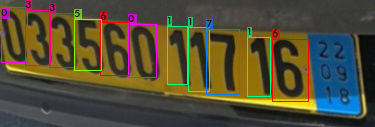
\includegraphics[width=0.9\textwidth]{predictions}
  \caption{Test figure}
\end{figure}


\blindtext

\chapter[Convolutional neural networks]{Neural networks variant: Convolutional neural networks}
\chapter{Application of CNN in object detection}

\blindtext \cite{AN19}

\begin{figure}[!htbp]
  \centering
  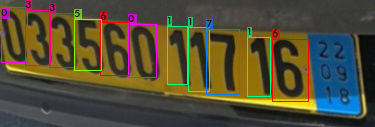
\includegraphics[width=0.9\textwidth]{predictions}
  \caption{Test figure}
\end{figure}


\blindtext

\section{R-CNN model}
\section{You Only Look Once model}

\blindtext

\begin{figure}[!htbp]
  \centering
  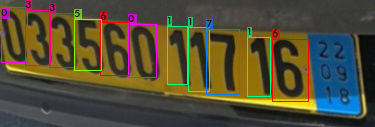
\includegraphics[width=0.9\textwidth]{predictions}
  \caption{Test figure}
\end{figure}


\blindtext \cite{2}

\chapter[Object detection in action]{Applying state-of-the-art CNNs to license plate recognition problem using preexisting implementations}

\begin{table}[h]
\centering % to center the table.
\caption{This is a table}
\begin{tabular}{@{}>{\itshape}ccc@{}}%since we have 3 characters we will have 3 columns and c stand for centered alignement
  % \hline % this creates a horizantal line % instead of using this we prefer the booktabs
  \toprule[1.5pt]
  \head{Command} & \head{Declaration} & \head{Output} \\
  \midrule
  list files     & ls                 & some files \\%[10pt]% to lavrage extra space
  change directoy     & cd                 & directory changed \\
  remove files and directories     & rm -r                 & file removed \\
  \bottomrule[1.5pt]

\end{tabular}
\end{table}

\section{Introduction to the licence plate problem}
\section{Discussing results}

\blindtext \cite{2}

\begin{table}[h]
\centering % to center the table.
\caption{This is a table}
\begin{tabular}{@{}>{\itshape}ccc@{}}%since we have 3 characters we will have 3 columns and c stand for centered alignement
  % \hline % this creates a horizantal line % instead of using this we prefer the booktabs
  \toprule[1.5pt]
  \head{Command} & \head{Declaration} & \head{Output} \\
  \midrule
  list files     & ls                 & some files \\%[10pt]% to lavrage extra space
  change directoy     & cd                 & directory changed \\
  remove files and directories     & rm -r                 & file removed \\
  \bottomrule[1.5pt]

\end{tabular}
\end{table}

\blindtext

\chapter[Object detection in action again]{Applying state-of-the-art CNNs to license plate recognition problem using preexisting implementations}

\section{brief implementations of both techniques}
\blindtext

\section{Integration of model in a desktop app}
\blindtext

\chapter{Real life applications}

\blindtext

\chapter*{Further imporvements}
\addcontentsline{toc}{chapter}{Further imporvements}
\blindtext

\chapter*{Conclusion}
\blindtext[5]
\addcontentsline{toc}{chapter}{Conclusion}
